\documentclass{standalone}
\usepackage{tikz}
\usetikzlibrary{patterns, positioning}

\begin{document}
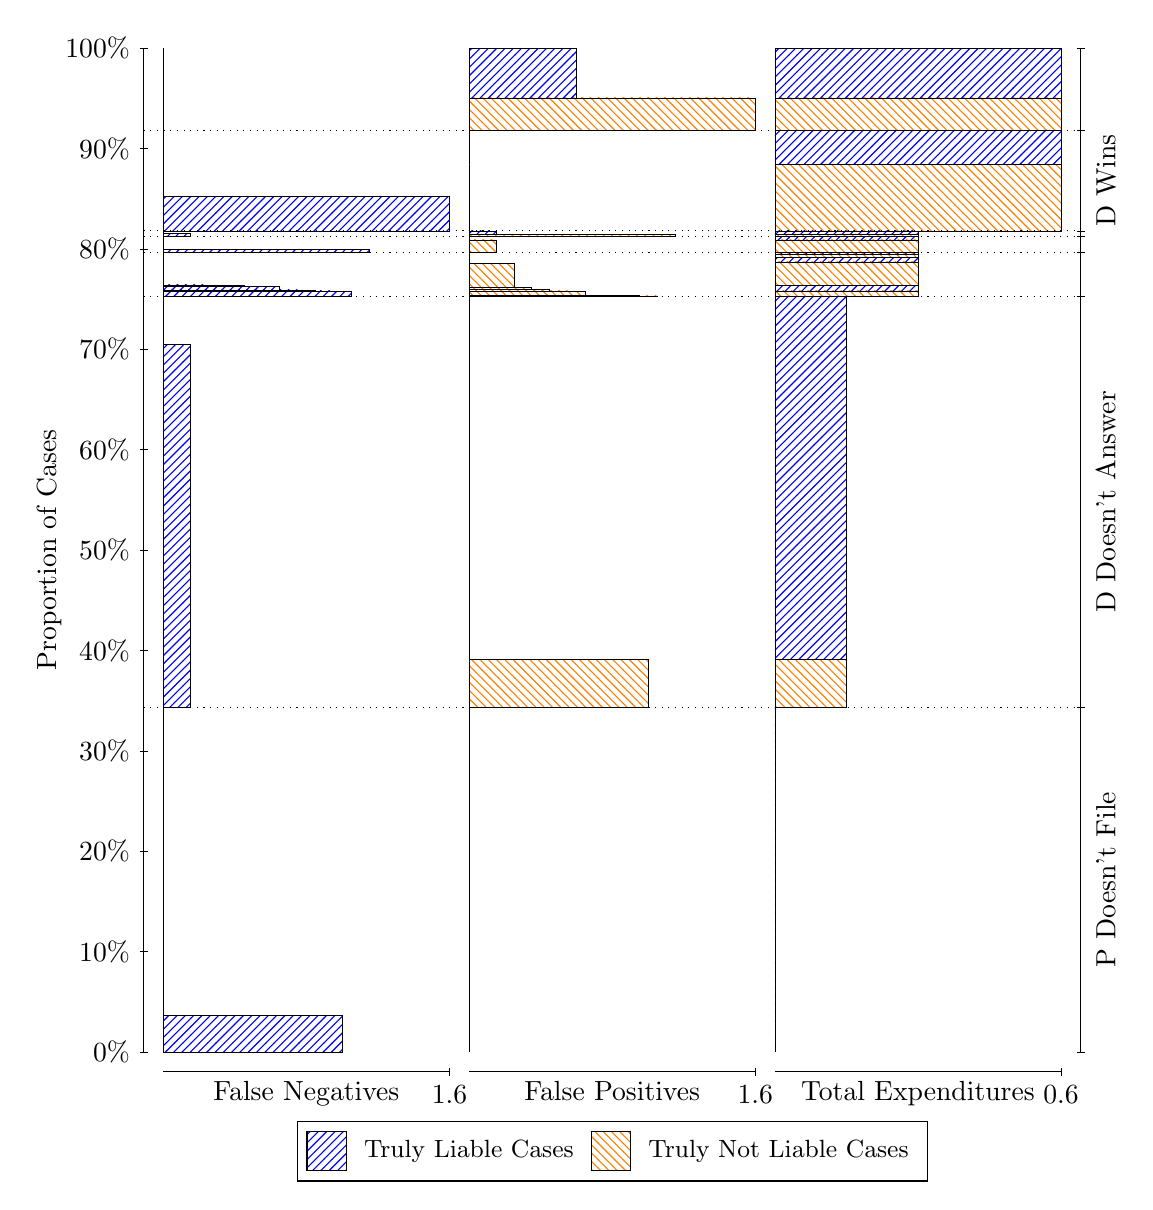
\begin{tikzpicture}
\draw[black, very thin] (1.5,1.75) -- (1.5,14.5);
\node[rotate=90, anchor=center] at (0.3, 8.125) {Proportion of Cases};
\draw[black, very thin] (1.45,1.75) -- (1.55,1.75);
\node[anchor=east] at (1.45, 1.75) {0\%};
\draw[black, very thin] (1.45,3.025) -- (1.55,3.025);
\node[anchor=east] at (1.45, 3.025) {10\%};
\draw[black, very thin] (1.45,4.3) -- (1.55,4.3);
\node[anchor=east] at (1.45, 4.3) {20\%};
\draw[black, very thin] (1.45,5.575) -- (1.55,5.575);
\node[anchor=east] at (1.45, 5.575) {30\%};
\draw[black, very thin] (1.45,6.85) -- (1.55,6.85);
\node[anchor=east] at (1.45, 6.85) {40\%};
\draw[black, very thin] (1.45,8.125) -- (1.55,8.125);
\node[anchor=east] at (1.45, 8.125) {50\%};
\draw[black, very thin] (1.45,9.4) -- (1.55,9.4);
\node[anchor=east] at (1.45, 9.4) {60\%};
\draw[black, very thin] (1.45,10.675) -- (1.55,10.675);
\node[anchor=east] at (1.45, 10.675) {70\%};
\draw[black, very thin] (1.45,11.95) -- (1.55,11.95);
\node[anchor=east] at (1.45, 11.95) {80\%};
\draw[black, very thin] (1.45,13.225) -- (1.55,13.225);
\node[anchor=east] at (1.45, 13.225) {90\%};
\draw[black, very thin] (1.45,14.5) -- (1.55,14.5);
\node[anchor=east] at (1.45, 14.5) {100\%};

\draw[black, very thin] (13.4,1.75) -- (13.4,14.5);
\draw[black, very thin] (13.35,1.75) -- (13.45,1.75);
\node[anchor=west] at (13.35, 1.75) {};
\draw[black, very thin] (13.35,6.1262) -- (13.45,6.1262);
\node[anchor=west] at (13.35, 6.1262) {};
\draw[black, very thin] (13.35,11.347) -- (13.45,11.347);
\node[anchor=west] at (13.35, 11.347) {};
\draw[black, very thin] (13.35,11.905) -- (13.45,11.905);
\node[anchor=west] at (13.35, 11.905) {};
\draw[black, very thin] (13.35,12.103) -- (13.45,12.103);
\node[anchor=west] at (13.35, 12.103) {};
\draw[black, very thin] (13.35,12.177) -- (13.45,12.177);
\node[anchor=west] at (13.35, 12.177) {};
\draw[black, very thin] (13.35,13.458) -- (13.45,13.458);
\node[anchor=west] at (13.35, 13.458) {};
\draw[black, very thin] (13.35,14.5) -- (13.45,14.5);
\node[anchor=west] at (13.35, 14.5) {};

\draw[black, very thin, pattern color=blue, pattern=north east lines] (1.75,1.75) rectangle (4.0208,2.2179);
\draw[black, very thin, pattern color=orange, pattern=north west lines] (1.75,2.2179) rectangle (1.75,6.1262);
\draw[black, very thin, pattern color=blue, pattern=north east lines] (1.75,6.1262) rectangle (2.0906,10.734);
\draw[black, very thin, pattern color=orange, pattern=north west lines] (1.75,10.734) rectangle (1.75,11.347);
\draw[black, very thin, pattern color=blue, pattern=north east lines] (1.75,11.347) rectangle (4.1344,11.407);
\draw[black, very thin, pattern color=blue, pattern=north east lines] (1.75,11.407) rectangle (3.9073,11.415);
\draw[black, very thin, pattern color=blue, pattern=north east lines] (1.75,11.415) rectangle (3.6802,11.425);
\draw[black, very thin, pattern color=blue, pattern=north east lines] (1.75,11.425) rectangle (3.4531,11.428);
\draw[black, very thin, pattern color=blue, pattern=north east lines] (1.75,11.428) rectangle (3.226,11.475);
\draw[black, very thin, pattern color=blue, pattern=north east lines] (1.75,11.475) rectangle (2.999,11.477);
\draw[black, very thin, pattern color=blue, pattern=north east lines] (1.75,11.477) rectangle (2.7719,11.481);
\draw[black, very thin, pattern color=blue, pattern=north east lines] (1.75,11.481) rectangle (2.5448,11.483);
\draw[black, very thin, pattern color=blue, pattern=north east lines] (1.75,11.483) rectangle (2.3177,11.491);
\draw[black, very thin, pattern color=orange, pattern=north west lines] (1.75,11.491) rectangle (1.75,11.905);
\draw[black, very thin, pattern color=blue, pattern=north east lines] (1.75,11.905) rectangle (4.3615,11.945);
\draw[black, very thin, pattern color=orange, pattern=north west lines] (1.75,11.945) rectangle (1.75,12.103);
\draw[black, very thin, pattern color=blue, pattern=north east lines] (1.75,12.103) rectangle (2.0906,12.145);
\draw[black, very thin, pattern color=orange, pattern=north west lines] (1.75,12.145) rectangle (1.75,12.177);
\draw[black, very thin, pattern color=blue, pattern=north east lines] (1.75,12.177) rectangle (5.3833,12.616);
\draw[black, very thin, pattern color=orange, pattern=north west lines] (1.75,12.616) rectangle (1.75,13.458);
\draw[black, very thin, pattern color=orange, pattern=north west lines] (1.75,13.458) rectangle (1.75,13.867);
\draw[black, very thin, pattern color=blue, pattern=north east lines] (1.75,13.867) rectangle (1.75,14.5);
\draw[black, very thin, pattern color=orange, pattern=north west lines] (5.6333,1.75) rectangle (5.6333,5.6583);
\draw[black, very thin, pattern color=blue, pattern=north east lines] (5.6333,5.6583) rectangle (5.6333,6.1262);
\draw[black, very thin, pattern color=orange, pattern=north west lines] (5.6333,6.1262) rectangle (7.9042,6.7395);
\draw[black, very thin, pattern color=blue, pattern=north east lines] (5.6333,6.7395) rectangle (5.6333,11.347);
\draw[black, very thin, pattern color=orange, pattern=north west lines] (5.6333,11.347) rectangle (8.0177,11.353);
\draw[black, very thin, pattern color=orange, pattern=north west lines] (5.6333,11.353) rectangle (7.7906,11.355);
\draw[black, very thin, pattern color=orange, pattern=north west lines] (5.6333,11.355) rectangle (7.5635,11.359);
\draw[black, very thin, pattern color=orange, pattern=north west lines] (5.6333,11.359) rectangle (7.3365,11.361);
\draw[black, very thin, pattern color=orange, pattern=north west lines] (5.6333,11.361) rectangle (7.1094,11.411);
\draw[black, very thin, pattern color=orange, pattern=north west lines] (5.6333,11.411) rectangle (6.8823,11.416);
\draw[black, very thin, pattern color=orange, pattern=north west lines] (5.6333,11.416) rectangle (6.8823,11.416);
\draw[black, very thin, pattern color=orange, pattern=north west lines] (5.6333,11.416) rectangle (6.6552,11.437);
\draw[black, very thin, pattern color=orange, pattern=north west lines] (5.6333,11.437) rectangle (6.4281,11.458);
\draw[black, very thin, pattern color=orange, pattern=north west lines] (5.6333,11.458) rectangle (6.201,11.761);
\draw[black, very thin, pattern color=blue, pattern=north east lines] (5.6333,11.761) rectangle (5.7469,11.769);
\draw[black, very thin, pattern color=blue, pattern=north east lines] (5.6333,11.769) rectangle (5.6333,11.905);
\draw[black, very thin, pattern color=orange, pattern=north west lines] (5.6333,11.905) rectangle (5.974,12.063);
\draw[black, very thin, pattern color=blue, pattern=north east lines] (5.6333,12.063) rectangle (5.6333,12.103);
\draw[black, very thin, pattern color=orange, pattern=north west lines] (5.6333,12.103) rectangle (8.2448,12.135);
\draw[black, very thin, pattern color=blue, pattern=north east lines] (5.6333,12.135) rectangle (5.974,12.177);
\draw[black, very thin, pattern color=orange, pattern=north west lines] (5.6333,12.177) rectangle (5.6333,13.019);
\draw[black, very thin, pattern color=blue, pattern=north east lines] (5.6333,13.019) rectangle (5.6333,13.458);
\draw[black, very thin, pattern color=orange, pattern=north west lines] (5.6333,13.458) rectangle (9.2667,13.867);
\draw[black, very thin, pattern color=blue, pattern=north east lines] (5.6333,13.867) rectangle (6.9958,14.5);
\draw[black, very thin, pattern color=orange, pattern=north west lines] (9.5167,1.75) rectangle (9.5167,5.6583);
\draw[black, very thin, pattern color=blue, pattern=north east lines] (9.5167,5.6583) rectangle (9.5167,6.1262);
\draw[black, very thin, pattern color=orange, pattern=north west lines] (9.5167,6.1262) rectangle (10.425,6.7395);
\draw[black, very thin, pattern color=blue, pattern=north east lines] (9.5167,6.7395) rectangle (10.425,11.347);
\draw[black, very thin, pattern color=orange, pattern=north west lines] (9.5167,11.347) rectangle (11.333,11.416);
\draw[black, very thin, pattern color=blue, pattern=north east lines] (9.5167,11.416) rectangle (11.333,11.482);
\draw[black, very thin, pattern color=orange, pattern=north west lines] (9.5167,11.482) rectangle (11.333,11.784);
\draw[black, very thin, pattern color=blue, pattern=north east lines] (9.5167,11.784) rectangle (11.333,11.844);
\draw[black, very thin, pattern color=orange, pattern=north west lines] (9.5167,11.844) rectangle (11.333,11.886);
\draw[black, very thin, pattern color=blue, pattern=north east lines] (9.5167,11.886) rectangle (11.333,11.905);
\draw[black, very thin, pattern color=orange, pattern=north west lines] (9.5167,11.905) rectangle (11.333,12.063);
\draw[black, very thin, pattern color=blue, pattern=north east lines] (9.5167,12.063) rectangle (11.333,12.103);
\draw[black, very thin, pattern color=orange, pattern=north west lines] (9.5167,12.103) rectangle (11.333,12.135);
\draw[black, very thin, pattern color=blue, pattern=north east lines] (9.5167,12.135) rectangle (11.333,12.177);
\draw[black, very thin, pattern color=orange, pattern=north west lines] (9.5167,12.177) rectangle (13.15,13.019);
\draw[black, very thin, pattern color=blue, pattern=north east lines] (9.5167,13.019) rectangle (13.15,13.458);
\draw[black, very thin, pattern color=orange, pattern=north west lines] (9.5167,13.458) rectangle (13.15,13.867);
\draw[black, very thin, pattern color=blue, pattern=north east lines] (9.5167,13.867) rectangle (13.15,14.5);
\draw[black, dotted] (1.5,6.1262) -- (13.4,6.1262);
\draw[black, dotted] (1.5,11.347) -- (13.4,11.347);
\draw[black, dotted] (1.5,11.905) -- (13.4,11.905);
\draw[black, dotted] (1.5,12.103) -- (13.4,12.103);
\draw[black, dotted] (1.5,12.177) -- (13.4,12.177);
\draw[black, dotted] (1.5,13.458) -- (13.4,13.458);
\draw[black, very thin] (1.75,1.5) -- (5.3833,1.5);
\node[anchor=north] at (3.5667, 1.5) {False Negatives};
\draw[black, very thin] (5.3833,1.45) -- (5.3833,1.55);
\node[anchor=north] at (5.3833, 1.45) {1.6};

\draw[black, very thin] (5.6333,1.5) -- (9.2667,1.5);
\node[anchor=north] at (7.45, 1.5) {False Positives};
\draw[black, very thin] (9.2667,1.45) -- (9.2667,1.55);
\node[anchor=north] at (9.2667, 1.45) {1.6};

\draw[black, very thin] (9.5167,1.5) -- (13.15,1.5);
\node[anchor=north] at (11.333, 1.5) {Total Expenditures};
\draw[black, very thin] (13.15,1.45) -- (13.15,1.55);
\node[anchor=north] at (13.15, 1.45) {0.6};

\node[black, centered, rotate=90] at (13.72, 3.9381) {P Doesn't File};
\node[black, centered, rotate=90] at (13.72, 8.7368) {D Doesn't Answer};



\node[black, centered, rotate=90] at (13.72, 12.817) {D Wins};


\draw (7.449999999999999,1.5) node[draw=none] (baseCoordinate) {};
\begin{scope}[align=center]
        \matrix[scale=0.5, draw=black, below=0.5cm of baseCoordinate, nodes={draw}, column sep=0.1cm]{
            \node[rectangle, draw, minimum width=0.5cm, minimum height=0.5cm, pattern=north east lines, pattern color=blue] {}; &
            \node[draw=none, font=\small] (B) {Truly Liable Cases}; &
            \node[rectangle, draw, minimum width=0.5cm, minimum height=0.5cm, pattern=north west lines, pattern color=orange] {}; &
            \node[draw=none, font=\small] (B) {Truly Not Liable Cases}; \\
            };
\end{scope}

\end{tikzpicture}
\end{document}